% This file was created with tikzplotlib v0.10.1.
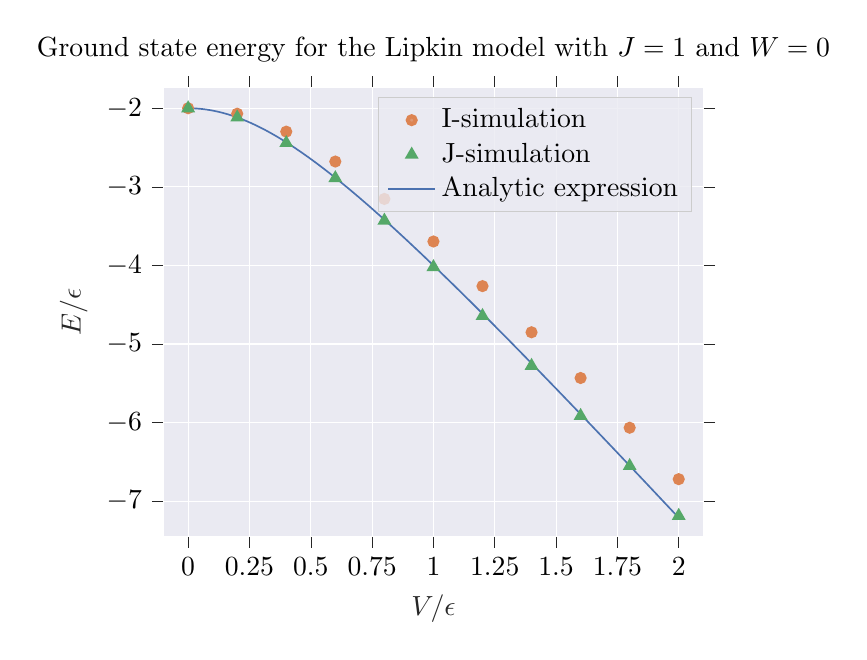
\begin{tikzpicture}

\definecolor{darkslategray38}{RGB}{38,38,38}
\definecolor{lavender234234242}{RGB}{234,234,242}
\definecolor{lightgray204}{RGB}{204,204,204}
\definecolor{mediumseagreen85168104}{RGB}{85,168,104}
\definecolor{peru22113282}{RGB}{221,132,82}
\definecolor{steelblue76114176}{RGB}{76,114,176}

\begin{axis}[
axis background/.style={fill=lavender234234242},
axis line style={white},
legend cell align={left},
legend style={
  fill opacity=0.8,
  draw opacity=1,
  text opacity=1,
  draw=lightgray204,
  fill=lavender234234242
},
mark options={mark size=1.4pt, line width=1.5pt},
minor xtick={},
minor ytick={},
tick align=outside,
title style={align=center},
title={Ground state energy for the Lipkin model with \(\displaystyle J = 1\) and \(\displaystyle W = 0\)},
x grid style={white},
xlabel=\textcolor{darkslategray38}{\(\displaystyle V/\epsilon\)},
xmajorgrids,
xmajorticks=false,
xmajorticks=true,
xmin=-0.1, xmax=2.1,
xtick style={color=darkslategray38},
xtick={-0.25,0,0.25,0.5,0.75,1,1.25,1.5,1.75,2,2.25},
y grid style={white},
ylabel=\textcolor{darkslategray38}{\(\displaystyle E/\epsilon\)},
ymajorgrids,
ymajorticks=false,
ymajorticks=true,
ymin=-7.44544014814064, ymax=-1.74069332627902,
ytick style={color=darkslategray38},
ytick={-8,-7,-6,-5,-4,-3,-2,-1}
]
\addplot [draw=peru22113282, fill=peru22113282, mark=*, only marks]
table{%
x  y
0 -2
0.2 -2.06966
0.4 -2.29776
0.6 -2.67806
0.8 -3.15404
1 -3.6955
1.2 -4.2633
1.4 -4.85082
1.6 -5.43256
1.8 -6.06534
2 -6.7198
};
\addlegendentry{I-simulation}
\addplot [draw=mediumseagreen85168104, fill=mediumseagreen85168104, mark=triangle*, only marks]
table{%
x  y
0 -2
0.2 -2.11737467780841
0.4 -2.44181795157578
0.6 -2.88888711699146
0.8 -3.42967172403921
1 -4.02057985967262
1.2 -4.64308141861071
1.4 -5.27699247400839
1.6 -5.91416751763876
1.8 -6.5519807970815
2 -7.18613347441966
};
\addlegendentry{J-simulation}
\addplot [semithick, steelblue76114176]
table {%
0 -2
0.00999999046325684 -2.00029993057251
0.0199999809265137 -2.00119972229004
0.0299999713897705 -2.00269818305969
0.0399999618530273 -2.00479435920715
0.0499999523162842 -2.00748610496521
0.059999942779541 -2.01077103614807
0.0700000524520874 -2.01464629173279
0.0800000429153442 -2.01910877227783
0.0900000333786011 -2.02415418624878
0.100000023841858 -2.02977824211121
0.110000014305115 -2.03597640991211
0.120000004768372 -2.04274320602417
0.139999985694885 -2.05796027183533
0.159999966621399 -2.07537937164307
0.180000066757202 -2.09494638442993
0.200000047683716 -2.11660099029541
0.220000028610229 -2.14028024673462
0.240000009536743 -2.16591787338257
0.259999990463257 -2.19344472885132
0.279999971389771 -2.22279095649719
0.299999952316284 -2.25388550758362
0.319999933242798 -2.28665685653687
0.340000033378601 -2.32103419303894
0.360000014305115 -2.35694718360901
0.379999995231628 -2.39432668685913
0.399999976158142 -2.43310499191284
0.430000066757202 -2.49375224113464
0.460000038146973 -2.55718588829041
0.490000009536743 -2.62320423126221
0.519999980926514 -2.69161653518677
0.549999952316284 -2.76224541664124
0.579999923706055 -2.83492493629456
0.620000004768372 -2.93475723266602
0.660000085830688 -3.03763055801392
0.700000047683716 -3.1432466506958
0.740000009536743 -3.2513382434845
0.789999961853027 -3.38957214355469
0.839999914169312 -3.53089213371277
0.889999985694885 -3.67494225502014
0.950000047683716 -3.8509738445282
1.00999999046326 -4.03003740310669
1.08000004291534 -4.24226331710815
1.14999997615814 -4.4575777053833
1.23000001907349 -4.7068886756897
1.30999994277954 -4.959153175354
1.39999997615814 -5.24595069885254
1.5 -5.56776428222656
1.61000001430511 -5.92496395111084
1.73000001907349 -6.31781625747681
1.86000001430511 -6.74649524688721
1.99000000953674 -7.17782688140869
};
\addlegendentry{Analytic expression}
\end{axis}

\end{tikzpicture}
